\chapter{Antecedentes}

A principios del milenio, el grupo GITEM inició un estudio para abordar problemas puntuales en la implementación de servicios médicos prestados a través de medios teleinformáticos en el Distrito Capital\cite{aparicio2000}:

\begin{quote}
“En el momento no existe un diagnóstico real sobre los servicios requeridos en el área de telemedicina, razón suficiente para iniciar un trabajo de campo que establezca la situación actual de servicios médicos y la demanda real, así como la posibilidad de conocer a corto, mediano y largo plazo cuáles serían los costos de inversión que permitirían dar soluciones al problema  de cobertura.

La socialización del conocimiento alrededor de las tecnologías aplicadas al desarrollo de la medicina, es uno de los valores que lleva al éxito de soluciones efectivas en el sector salud, por tal motivo es necesario desarrollar un plan de alfabetización en el sector salud y en el sector gubernamental y académico.

En el país no existen estrategias de investigación en esta área del conocimiento para llevar a cabo un estudio real que permita dar el paso a soluciones verdaderas sobre desarrollo tecnológico o experimental para poder implementar centros de investigación en Telemedicina.

La Universidad Distrital tiene el recurso humano, el conocimiento y la experiencia científica y tecnológica, capaz de dar soluciones tangibles a estas necesidades; unida al conocimiento y experiencia de entidades como clínicas y hospitales  y con la participación de operadores de comunicaciones, puede desarrollar soluciones efectivas a los problemas de salud que afronta la sociedad colombiana.”
\end{quote}

Para facilitar el aprovechamiento del estudio, los resultados obtenidos fueron recopilados en extensos tomos en formato físico y digital. Aunque eficaz en primera instancia, los resultados obtenidos no tenían una estructura documental coherente ni un modelo de información que los caracterizara. Este hecho, a la par con el ingreso de entidades al estudio, aumentó la complejidad a la hora de generar estudios comparativos o de apoyo a la toma de decisiones, teniéndose en muchos casos información faltante, redundante e innecesaria para el proyecto. Dado que la muestra objeto de estudio es intrínsecamente dinámica, cualquier cambio de la condiciones iniciales es difícilmente reflejado, quedando en poco tiempo la información desactualizada. En ese escenario, la labor de articular las prestaciones de las organizaciones suponía un proceso lento y la estrategia de gestión de información empleada en el estudio comenzó a mostrar debilidades.

Respondiendo a este nuevo contexto problémico se creó al interior del grupo un proyecto denominado \textbf{Sistema de Información para la Caracterización de Proyectos de eSalud}, que en sus primeras fases de desarrollo dio solución parcial al marcar las pautas hacia la integración de información para el \textbf{GITEM}. En paralelo el grupo de investigación implementó, en convenio con \textit{Colciencias}, el Sistema de Referencia y Contrarreferencia para el Distrito Capital, utilizando herramientas de desarrollo propietarias específicamente el middleware .NET de Microsoft con lo que el grupo adquirió experiencia en la desarrollo de aplicaciones siguiendo metodologías efectivas para la construcción de software.

\section{Sistema de Información para la Caracterización de Proyectos de eSalud}

Problemas asociados con malas interpretaciones del concepto de \textit{licencia a perpetuidad} del software propietario, plantearon la necesidad de realizar investigación relacionada con el desarrollo de software distribuido, interoperable y robusto basado en la filosofía del software libre y del código abierto- es decir, que abordara sus potencialidades y encarara sus debilidades en un entorno de trabajo de corte industrial. Bajo este enfoque nació SITEM.

SITEM es un proyecto de investigación asociado a un holotipo proyectivo\cite{hurtado2000}, que tiene como impacto esperado el apoyo a labores de consultoría y diseño de redes de eSalud. Se desarrolla con un método de trabajo que surge de la metodología de OpenUP\cite{balduino2010} en donde se prioriza las disciplinas de Requisitos y Arquitectura, teniendo en cuenta el riesgo que se tiene en el grupo de investigación para consolidar equipos de trabajo por periodos de tiempo superiores a tres meses.

El proyecto tiene como particularidad el tener que cumplir con los requisitos empleando reducidos recursos técnicos y financieros, los cuales deben ser administrados dentro de un ambiente de alta regulación burocrática. El escenario común ha sido el bajo tiempo de permanencia de los integrantes, la ejecución constante de tareas de capacitación, el uso intensivo de tecnologías de la comunicación, el teletrabajo  y la escasa interacción persona a persona. Con nuestra experiencia comprobamos la máxima de Larman \cite{larman2003} : “Rápido, barato, bueno: elija dos cualquiera”; y dejando a un lado las fuertes esperanzas, sacrificamos el único aspectos que podíamos y la rapidez en que versiones estables del proyecto habrían de ver la luz se reduciría significativamente. No obstante, los conceptos fundamentales de desarrollo de aplicaciones de software libre \cite{raymond} han aportado varias claves para minimizar el impacto de este sacrificio.

\begin{figure}
 \centering
 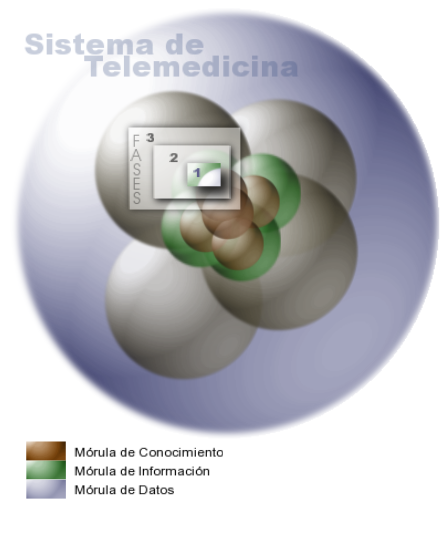
\includegraphics[width=156mm, height=195mm]{modelo_fases.png}
 \caption{Aproximación incremental a un sistema de Gestión de Conocimiento}
 \label{modelo1}
\end{figure}

El grupo plantea un modelo general en donde los objetivos de producir datos, consumir información y compartir conocimiento en el área de interés, será alcanzado en varias fases\footnote{A través del presente documento se utilizan los términos de fase en el proceso investigativo y fases del Proceso de Desarrollo del Sistema Software. Las dos se suponen diferentes y su interpretación e importancia están asociados al contexto en el que se ubican.} de las cuales este documento describe aquellas que han culminado.

La figura \ref{modelo1} muestra el proceso de estructuración del sistema como una sucesión de fases que generan dimensiones de datos, información y conocimiento de un componente. El sistema visto como un \textit{holos} presenta al investigador una gran cantidad de datos que en la medida que se descubren, recolectan, observan y registran se vuelven susceptibles de ser descritos, analizados, integrados y comparados (información), acercándose a un conocimiento refinado. El carácter de discernible - el momento en que las dimensiones se solapan en grado sumo, se evidencia con el aumento colectivo de especialización en la materia y en nuestro caso, con el grado de inmersión que los usuarios del SITEM tengan a partir de la liberación de la versión 1.0 estable (diciembre de 2017).

En el transcurso de las fases \textit{solo se manejan ciertos aspectos} que incrementalmente refinan el modelo del sistema, con base en las diferentes \textit{mórulas} de datos, información y conocimiento generadas. Aunque en el gráfico se muestra un tanto discretos y exactos, los límites existentes entre las tres mórulas principales - datos, información, conocimiento; son en la realidad difusos. Si se consideran los aspectos meramente técnicos del SITEM se corre el riesgo inminente de diseminación en regiones poco profundas del sistema - dispersión en la mórula de datos - razón por la cual la herramienta software se ha convertido en un artefacto intermedio y no en el fin último de la investigación.

\subsection{SITEM – Fase I}
Con la primera fase  se definió un conjunto base de componentes de las redes de eSalud y sus interrelaciones, basado en una investigación exploratoria y descriptiva realizada por los integrantes del grupo. También se determinaron las características esenciales del portal esperado para el SITEM vislumbrando la necesidad de integrar un producto software adaptado a las necesidades del entorno distrital. Esto teniendo en cuenta que no existe una plataforma de acceso público que permita la gestión y análisis de información pertinente, confiable, actualizada y estructurada en torno a las redes de eSalud del Distrito Capital.

Esta fase se definió un modelo de negocios que lograba mostrar las interrelaciones que tendría el sistema con los proyectos del grupo y un conjunto representativo de portales relacionados temáticamente, encontrando \textit{un costo de oportunidad adecuado ya que en la actualidad ningún portal se especializa en el proceso de diagnóstico de capacidad para la implementación de eSalud.} No obstante, al momento de emprender el desarrollo, el grupo de investigación no contaba con los recursos mínimos requeridos por lo cual la propuesta y su implementación no pasó de ser un prototipo de baja funcionalidad. 

Los alcances y logros efectivos de esta fase fueron:

\begin{itemize}
\item Descripción del Modelo de Negocio.
\item Propuesta de Desarrollo.
\item Bosquejo de la Arquitectura general del Sistema.
\item Integración conceptual del SITEM dentro de los proyectos del grupo.
\item Estudios sobre filosofía de Software Libre y el movimiento del código abierto.
\item Construcción de un Prototipo de baja funcionalidad conocido como SITEM versión 0.1, bautizada internamente como \textbf{Kauil}.
\end{itemize}


\begin{figure}
 \centering
 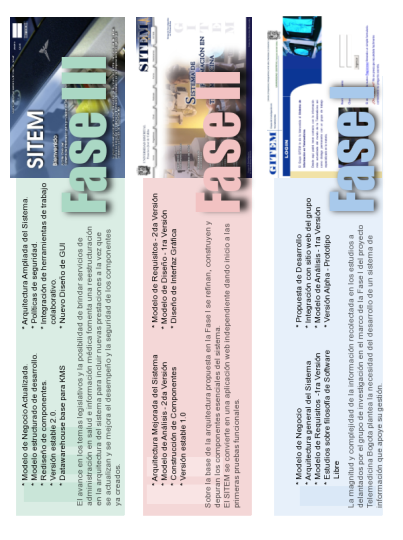
\includegraphics[width=142mm, height=190mm]{fase_sitem.png}
 \caption{Fases transcurridas en el desarrollo del SITEM}
 \label{fase_sitem}
\end{figure}

\subsection{SITEM – Fase II}

El modelo de negocio y el modelos de requisitos, análisis y diseño sirvieron de base para la segunda fase cuyo objetivo era \textit{..describir una arquitectura general para el Sistema de Información para la Caracterización de Proyectos de eSalud}; y crear un portal prototipo que integrara componentes de software para concretar parte de dicha arquitectura. Para poder minimizar los riesgos asociados al proyecto se adaptó el \textit{OpenUP} a las especificidades de desarrollo del Sistema, lo que favoreció efectivamente su elaboración, implementación, mantenimiento y crecimiento.

En la segunda fase, debido a la naturaleza del SITEM, el grupo de investigación decide separar los hilos de desarrollo del Sistema y del proceso de estructuración del sitio web del grupo. El SITEM por primera vez se puede acceder desde \textit{Internet} gracias al despliegue que se realiza sobre la plataforma de hardware y software brindada por la \textit{Universidad Distrital}. 

En esta fase se realiza el modelado de datos y se esbozan las rutinas de manejo de seguridad. Para la integración de componentes se utilizan herramientas de software libre y el grupo de desarrollo aumenta a cinco integrantes. El trabajo se encuentra, con excepción del director del proyecto, soportado y ejecutado por estudiantes de pregrado del proyecto curricular de Ingeniería Electrónica convirtiéndose en el \textbf{primer proyecto de desarrollo de software libre realizado por el GITEM}.

Los alcances de esta fase fueron:
\begin{itemize}
\item Arquitectura Mejorada del Sistema
\item Modelo depurado de Requisitos
\item Modelo de Análisis - Segunda Versión
\item Modelo de Diseño
\item Construcción de Componentes software soportado en su totalidad por herramientas de software libre.
\item Versión 0.5 beta bautizada internamente como \textbf{Gucumatz}.
\end{itemize}


\subsection{SITEM – Fase III}

En esta fase el grupo toma una decisión arquitectónica importante y concentra su esfuerzo en el motor de integración de aplicaciones, cuyo objetivo es la federación de sistemas existentes de software libre o código abierto (FLOSS) con el objetivo de lograr un mayor nivel funcional del que se había alcanzado en las fases anteriores. Se trata de buscar el aseguramiento de la calidad en el desarrollo, la interoperabilidad, escalabilidad y el uso extensivo de FLOSS. Se documenta todas las etapas involucradas en la creación de la aplicación para que sirva de plantilla a sistemas relacionados y se formaliza las áreas de capacitación a partir de ciclos genéricos de transferencia de conocimiento apoyados en tecnologías de la información.

Es precisamente esta fase la que da vida a este documento, a una arquitectura emergente y una versión 1.0 del sistema denominada \textit{OpenSITEM}, con la que el grupo entrega un sistema complejo constituido por un motor de federación - basado en SARA un framework de desarrollo para aplicaciones web desarrollado por el grupo - que articula las herramientas externas Knowage, ERPNext, Alfresco Community, CAMUNDA y OpenProject, así como varias herramientas propias tales como:

\begin{itemize}
\item Sistema Integrado de Evaluación
\item Sistema de Gestión de Redes de Práctica y Colaboración
\item Sistema de agentes notificadores y de recomendación
\item Sistema de Información Geográfica 3D basado en Cesium.
\end{itemize}

De esta forma SITEM se convierte en una compleja solución que abarca diferentes dominios, con capacidad de adaptación para un propósito específico. En particular, la fase III se concentra en la configuración de OpenSITEM como \textit{Sistema de Información para la Caracterización de Proyectos de eSalud}.


\begin{figure}
 \centering
 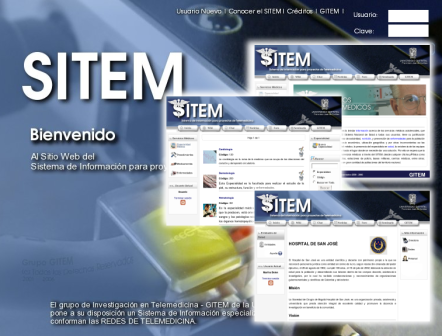
\includegraphics[width=156mm, height=118mm]{pagina_principal.png}
 \caption{Sistema de Información para la Caracterización de Proyectos de eSalud. Interfaz de Usuario en la Fase III}
 \label{sitem_faseIII}
\end{figure}